% !TeX root = main.tex

\documentclass[a4paper,12pt]{article}
\usepackage{bookmark}
% Import packages
\usepackage[margin=3cm]{geometry}
\usepackage[utf8]{inputenc}
\usepackage{amsmath}
\usepackage{subfig}
\usepackage{lingmacros}
\usepackage{tree-dvips}
\usepackage{fancyhdr}
\usepackage{listings}
\usepackage{subfig}
\usepackage{amsmath,amssymb}
\usepackage{lmodern}
\usepackage{iftex}
\usepackage{subfloat}
\usepackage{floatrow}
\usepackage{float}
\usepackage{xcolor}
\usepackage{geometry}
\usepackage{graphicx}
\usepackage{wrapfig}
\usepackage{amsmath}
\usepackage{hyperref}
\usepackage{floatrow}
\usepackage{float}
\usepackage{amssymb}
\usepackage{graphicx}
\usepackage{array}
\usepackage{booktabs}
\usepackage{algorithm} 
\usepackage{algpseudocode} 
\usepackage{subcaption}
\usepackage[T1]{fontenc}
\usepackage{stix}
\DeclareUnicodeCharacter{0360}{\eth}
%% papir layout
\geometry{
a4paper,
total={170mm,257mm},
left=15mm,
top=20mm,
}
\usepackage{tipa}
%% Layout og farve til hyperlinks
\definecolor{link}{rgb}{0,0,215}
\hypersetup{
    colorlinks=true,
    linkcolor=link,
    filecolor=link,      
    urlcolor=link,
    citecolor=black,
    pdfpagemode=FullScreen,
}

\usepackage[table]{xcolor}
\usepackage{fancyhdr}

%% Code style
\definecolor{comment}{rgb}{0,0.45,0}
\definecolor{codegray}{rgb}{0.5,0.5,0.5}
\definecolor{codepurple}{rgb}{0.58,0,0.82}
\definecolor{backcolour}{rgb}{0.95,0.95,0.92}
\lstdefinestyle{CodeStyle}{
    backgroundcolor=\color{backcolour},   
    commentstyle=\color{comment},
    keywordstyle=\color{magenta},
    numberstyle=\tiny\color{codegray},
    stringstyle=\color{codepurple},
    basicstyle=\ttfamily\footnotesize,
    breakatwhitespace=false,         
    breaklines=true,                 
    captionpos=b,                    
    keepspaces=true,                 
    numbers=left,                    
    numbersep=5pt,                  
    showspaces=false,                
    showstringspaces=false,
    showtabs=false,                  
    tabsize=2
}
\lstset{style=CodeStyle}
\lstdefinelanguage{JavaScript}{
  keywords={typeof, new, true, false, catch, function, return, null, catch, switch, var, if, in, while, do, else, case, break},
  keywordstyle=\color{purple}\bfseries,
  ndkeywords={class, export, const, var, let, boolean, throw, implements, import, this, !!, !=, ===, ;},
  ndkeywordstyle=\color{blue}\bfseries,
  identifierstyle=\color{black},
  sensitive=false,
  comment=[l]{//},
  morecomment=[s]{/*}{*/},
  commentstyle=\color{comment}\ttfamily,
  stringstyle=\color{orange}\ttfamily,
  morestring=[b]',
  morestring=[b]"
}

%% display \code{..}
\definecolor{light-gray}{gray}{0.95}
\newcommand{\code}[1]{\colorbox{light-gray}{\texttt{#1}}}
\usepackage{tocloft} \setlength\cftparskip{-5.5pt}

%% Litteraturliste
\usepackage[sorting=none]{biblatex}
\addbibresource{main.bib}
\newcommand{\class}[1]{\textbf{#1}}

\newcommand{\interface}[1]{\textit{#1}}

\newcommand{\aclass}[1]{\textbf{\underline{#1}}}

\newcommand{\package}[1]{\textit{\underline{#1}}}

\newcommand{\method}[1]{\textbf{\textit{#1}}}

\newcommand{\charactercount}[1]{
    \immediate\write18{
        expr `texcount -1 -sum -inc #1.tex` + `texcount -1 -sum -inc -char #1.tex` - 1 > chars.txt
    }\input{chars.txt}
}
\usepackage{graphicx} % Required for inserting images
\usepackage{comment}
\usepackage{float}
\usepackage{color}
\usepackage{hyperref}
\usepackage{geometry}
%\usepackage[danish]{babel}

\linespread{1.5} 

\hypersetup{
    colorlinks=true, %set true if you want colored links
    linktoc=all,     %set to all if you want both sections and subsections linked
    linkcolor=black,  %choose some color if you want links to stand out
}

\geometry{
 top=25mm,
}
\begin{document}
\setcounter{tocdepth}{2}
% Title page
\begin{center}
    \huge{\textbf{Minion Map}}\\
    \begin{figure}[ht]%
  \centering
  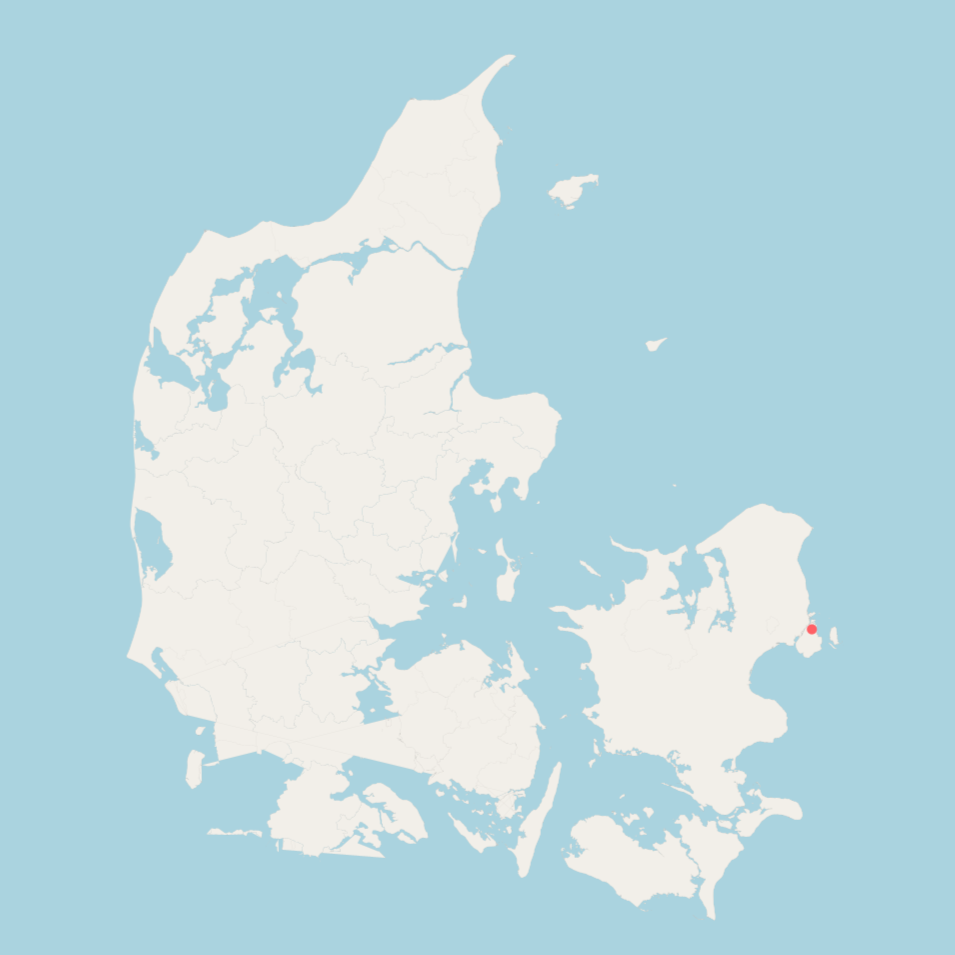
\includegraphics[width=11.5cm]{docs/material/Denmark_Photo.png}%
    \end{figure}\\
    \Large{Group 11.}\\
  \end{center}
  \begin{center}
    \begin{tabular}{p{2.85in}|p{2.85in}}
      Johannes Jørgensen & jgjo@itu.dk  \\   
      Elias Lindholdt & lild@itu.dk  \\
      Andreas Løvsgren Nielsen & anln@itu.dk\\
      Marius Cornelius Wisniewski Larsen & coml@itu.dk \\
      Kevin Skovgaard Gravesen & kegr@itu.dk \\    
      \hline
    \end{tabular}
  \end{center}
  \vspace{0.5cm}
  \begin{center}
    \vspace{0.5cm}
    First-Year Project, Bachelor in Software Development, IT Univ. of Copenhagen\\
    BSFDVNS1KU\\
    May 14, 2024
  \end{center}
\newpage
% header and footer
\pagestyle{fancy}
\fancyhead{} % clear all header fields
\fancyhead[RO,LE]{\textbf{Map of Denmark}}
\fancyhead[LO,RE]{\textbf{First Year Project}}
\fancyfoot{} % clear all footer fields
\fancyfoot[LE,RO]{\thepage}
\fancyfoot[LO,CE]{Group 11.}
\fancyfoot[CO,RE]{IT-University of Copenhagen}
\renewcommand*\contentsname{Table of Contents}
\tableofcontents
\newpage

\section{Preface}
During a 10 week period, the Geographic Information System (GIS) called “Minion Map” was developed as part of the `First Year Project: Map Of Denmark` course at the IT-University of Copenhagen. Minion Map was developed using Java and the graphics Library JavaFX.
This article aims to communicate the thought process and design choices throughout the development of Minion Map. 

\section{Introduction}
For millennia, humans have understood and recognised the importance and utility of maps and cartography. The history of mapping can be dated back more than 5.000 years, where humans would map places of interest on clay tablets or delicate maps on silk. In the modern era satellite systems, surveying techniques and contemporary cartographers are used to map the earth with very high precision and consistency. \cite*{littertur/icsm}
This has as a result made the cartographic data of the earth widely available to the general public, both from web-map services such as Google Maps and Apple Maps or from open source databases as OpenStreetMap.com. \\
\linebreak
While there already exists an abundance of digital maps, they generally adhere to many common features and design standards. Developing a straightforward and user-friendly digital map demands a substantial amount of coding and attentive use of algorithms and data structures. 

\subsection{Data set} \label{DataSet}
Minion Map uses data from the online cartographic database OpenStreetMap.com. The data is uploaded and maintained by volunteers worldwide, and is freely available to the public.\cite*{osm} 
The data comes in the form of .OSM files that are written in XML format, which contain all the necessary data needed to compile and run Minion Maps.
\par	The .OSM data consists of three data elements, which is nodes, ways and relations.   
\\Each of the three elements consist of a unique id, but the data elements have different structure for their data.\cite*{osm/XMLReader-Writer}
\newpage
\begin{itemize}
    \item Nodes(TagNode): A node is a pair of latitude and longitude.
    \item Ways(TagWay): A way comprises a list of at least two reference nodes, describing a linear feature. Closed ways exhibit identical first and last reference nodes. 
    \item Relations(TagRelation): Relations are a group of zero or more data elements with an associated role. 
\end{itemize}
All of the three data elements can contain a sub-data element named \textit{Tag}s, which can describe additional information about the data element.  
\subsection{Requirements} \label{Introduction/Requirements}
Through the project description, from our course BFST F2024, we were given a set of specific requirements that our final product have to include [A.1].
The formal requirements were then processed, interpreted and split up into the following system- and user-based requirements.
\subsubsection{System-Based Requirements}
\begin{enumerate}
\setlength{\itemsep}{0.1em}
    \item Compatibility for the “.zip” format, included default file for the program to use out of the box.
    \item Drawing roads different from what type they are.
    \item Graphical illustration of the map data contained within the bounds of a given rectangle chosen by the user.
    \item Showing the current zoom level.
    \item Multiple color themes for the user to pick from.
    \item Dynamic layout listening to window changes.
    \item Allowing address search.
    \item Pathfinding.
    \item Allowing the user to have multiple choices of transportation and allowing the user to place point of interests.
\end{enumerate}
\newpage
\subsubsection{User-Based Requirements}
\begin{enumerate}
    \setlength{\itemsep}{0.1em}
    \item Ensuring a clean GUI which is reasonably easy to navigate in and be fast enough for convenient use. 
    \item All of the system requirements will be developed having the user-based requirements in mind and by that not interfering with their fulfillment.
    \item By having the User-based requirements in mind, we gave ourselves some informal requirements for the final product. These include autocompletion of addresses in the searchmenu, the color scheme of the map shall be simple and clear, and all of the fulfilled requirements should be supported by a simple GUI.
    \item The formal and informal requirements prompt a multitude of different problems with the modern hardware and the chosen language, which we will try to solve with our final product.
\end{enumerate}


\section{Technical Design \& Analysis}
META TEXT NEEDED!!!\\
!!!\\
\subsection{Interface}
\subsection{Mecator Projection}
\subsection{Zoombar}
\section{Algorithms \& Data Structures}
\subsection{KDTree}
\subsection{Trie}
\subsection{Minimum Priority Queue}
\subsection{Pathfinding}

\section{Technical Description of the application}
\subsection{Considerations}
\subsection{Application Structure}
\subsection{Data Flow}
\subsubsection{Parser}
\textbf{TagBound}\\
\textbf{TagNode}\\
\textbf{TagWay}\\
\textbf{TagAddress}\\
\textbf{TagRelation}\\
\subsubsection{Data Processing}

 
\addcontentsline{toc}{section}{References}

\printbibliography[title={References}]

\end{document}